%%%%%%%%%%%%%%%%%%%%%%%%%%%%%%%%%%%%%%%%%%%%%%%%%%%%%%%%%%%%%%%%%%%%%%%%%%%%%%%%
\section{Quantum neural networks}
%%%%%%%%%%%%%%%%%%%%%%%%%%%%%%%%%%%%%%%%%%%%%%%%%%%%%%%%%%%%%%%%%%%%%%%%%%%%%%%%
\subsection{Hybrid quantum--classical computation}
%%%%%%%%%%%%%%%%%%%%%%%%%%%%%%%%%%%%%%%%%%%%%%%%%%%%%%%%%%%%%%%%%%%%%%%%%%%%%%%%
\begingroup
\nologo
\begin{frame}{Concept of hybrid computation}
	\centering
	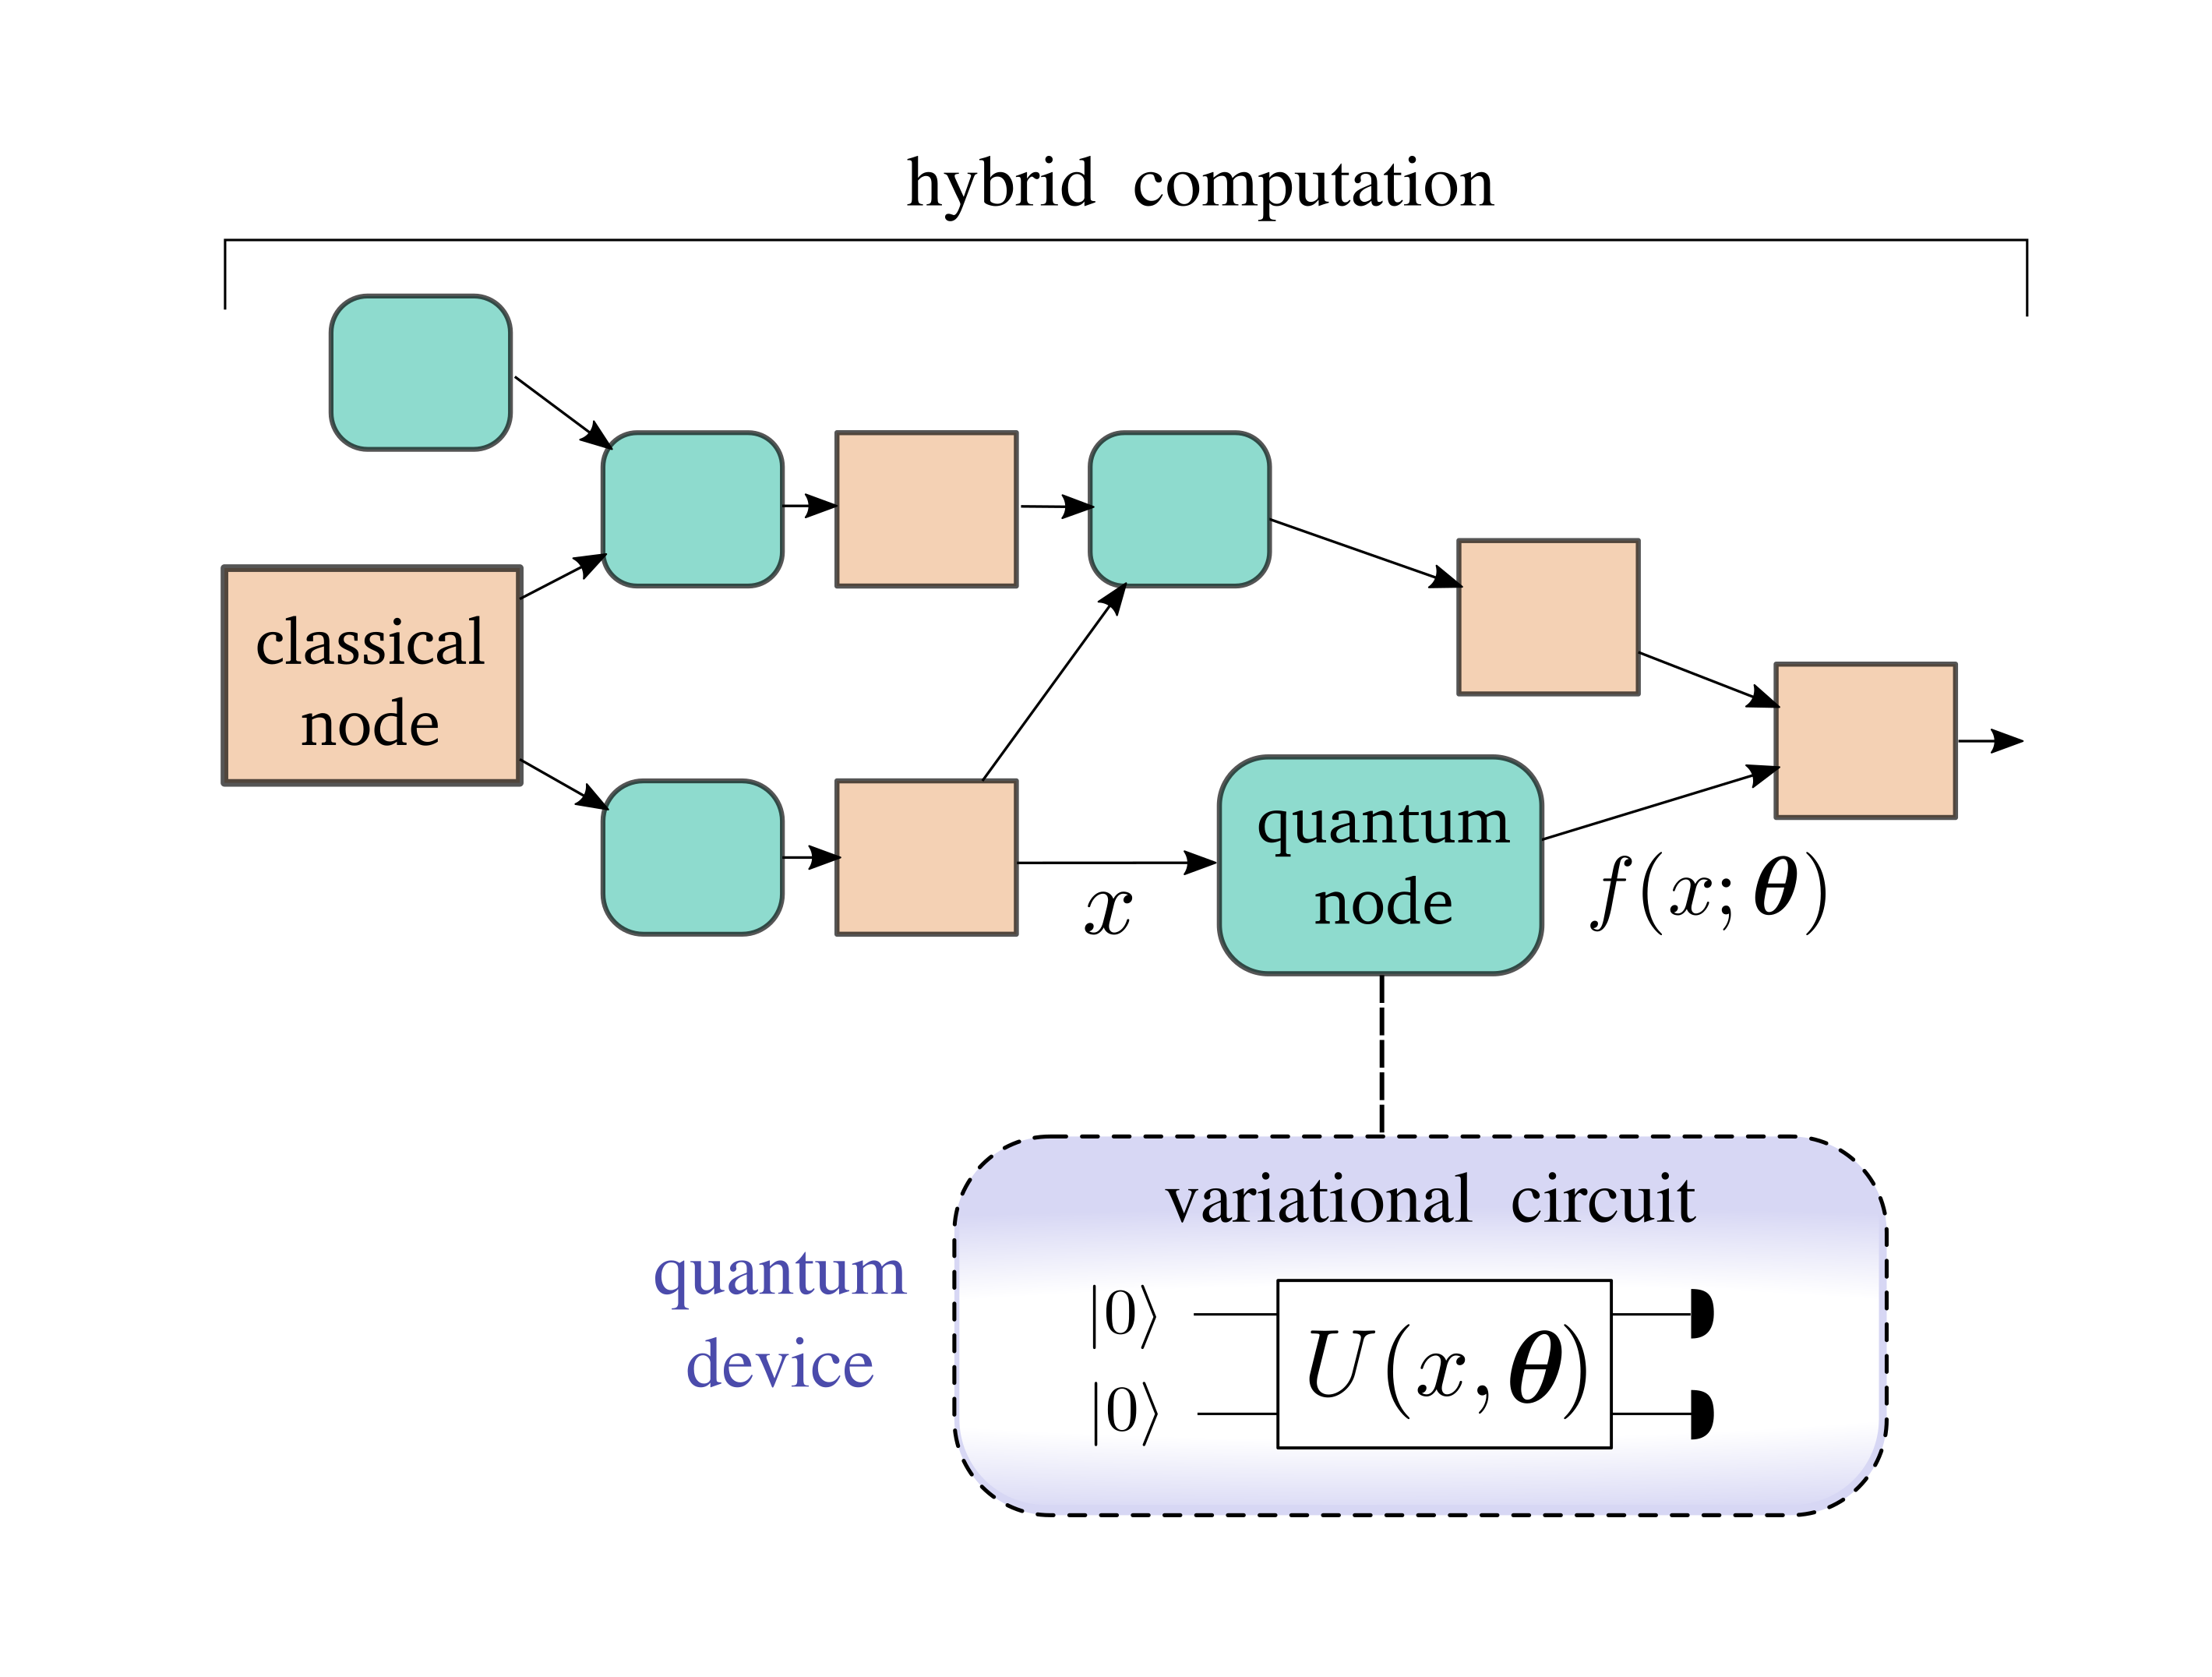
\includegraphics[height=0.8\textheight]{pics/vqc/concepts.png}
	\source{\url{https://github.com/XanaduAI/pennylane/} (Distributed under Apache Licence 2.0)}
\end{frame}
\endgroup
%%%%%%%%%%%%%%%%%%%%%%%%%%%%%%%%%%%%%%%%%%%%%%%%%%%%%%%%%%%%%%%%%%%%%%%%%%%%%%%%
\begingroup
\nologo
\begin{frame}{Gradient --- parameter shift rule}
	\centering
	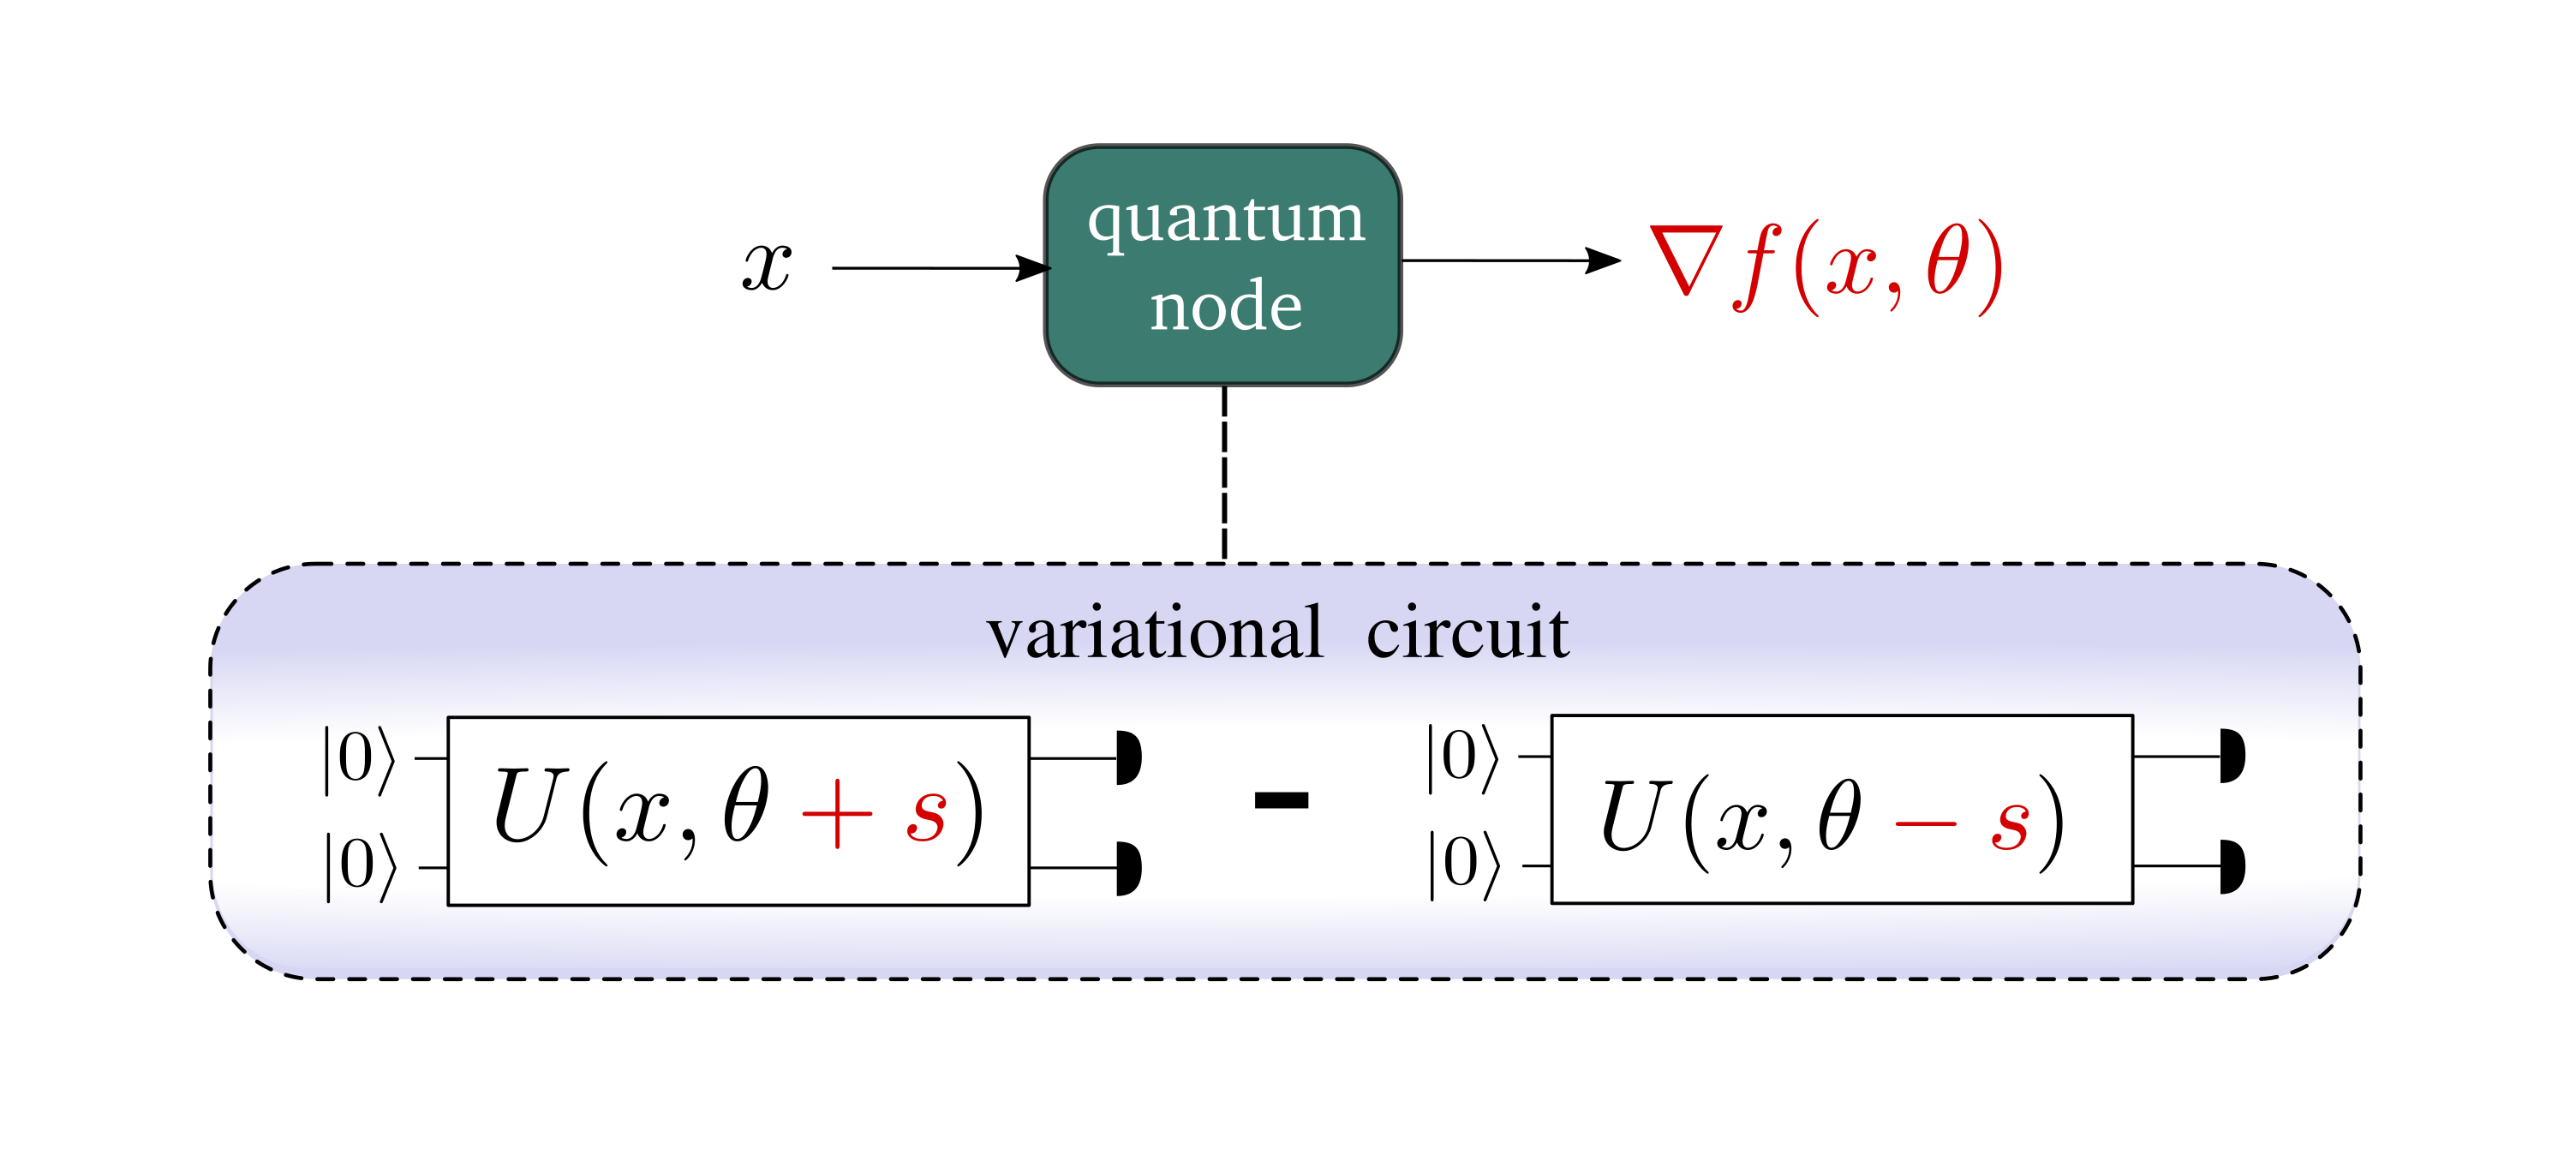
\includegraphics[height=0.75\textheight]{pics/vqc/grad.png}
	\source{\url{https://github.com/XanaduAI/pennylane/} (Distributed under Apache Licence 2.0)}
\end{frame}
\endgroup
%%%%%%%%%%%%%%%%%%%%%%%%%%%%%%%%%%%%%%%%%%%%%%%%%%%%%%%%%%%%%%%%%%%%%%%%%%%%%%%%
\subsection{Variational quantum circuits}
%%%%%%%%%%%%%%%%%%%%%%%%%%%%%%%%%%%%%%%%%%%%%%%%%%%%%%%%%%%%%%%%%%%%%%%%%%%%%%%%
\begin{frame}{Variational quantum circuit}
    \centering
    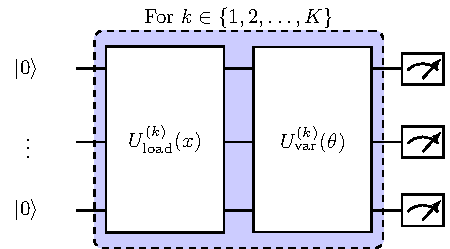
\includegraphics[width=0.9\textwidth]{pics/qnn/variational_circuit.pdf}
\end{frame}
%%%%%%%%%%%%%%%%%%%%%%%%%%%%%%%%%%%%%%%%%%%%%%%%%%%%%%%%%%%%%%%%%%%%%%%%%%%%%%%%
\subsection{Quantum neural network}
%%%%%%%%%%%%%%%%%%%%%%%%%%%%%%%%%%%%%%%%%%%%%%%%%%%%%%%%%%%%%%%%%%%%%%%%%%%%%%%%
\begin{frame}{Classification with Quantum Neural Network}
    \begin{block}{Data encoding}
        A data sample
        $$x=(x_1, x_2, \ldots, x_N)$$
        is encoded into a quantum state $\ket{x}$.
    \end{block}
    \begin{center}
        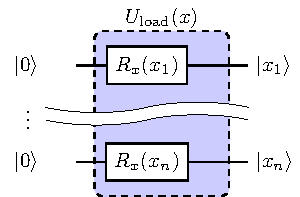
\includegraphics{pics/qnn/data_load.pdf}    
    \end{center}
\end{frame}    
%%%%%%%%%%%%%%%%%%%%%%%%%%%%%%%%%%%%%%%%%%%%%%%%%%%%%%%%%%%%%%%%%%%%%%%%%%%%%%%%
\begin{frame}{Classification with Quantum Neural Network}
    \begin{block}{Variational gate}
        A variational gate $U_{\mathrm{var}}(\theta)$ represents transformation of
        data by our quantum neural network.
    \end{block}
    \begin{center}
        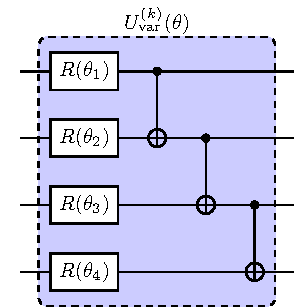
\includegraphics[scale=0.9]{pics/qnn/variational_ansatze.pdf}
    \end{center}
\end{frame}
%%%%%%%%%%%%%%%%%%%%%%%%%%%%%%%%%%%%%%%%%%%%%%%%%%%%%%%%%%%%%%%%%%%%%%%%%%%%%%%%
\subsection{Mathematical tools of QNNs}
%%%%%%%%%%%%%%%%%%%%%%%%%%%%%%%%%%%%%%%%%%%%%%%%%%%%%%%%%%%%%%%%%%%%%%%%%%%%%%%%
\begin{frame}{Observable, expectation value}
	\begin{itemize}
		\item Let $O$ be an \textbf{observable}---a quantum measurement whose labels
		are real numbers. 
		\item Mathematically it is represented as a Hermitian operator i.e.
		$$O^\dagger = O.$$ 
		\item The \textbf{expectation value} of an observable $O$ in
		a state $\ket{\psi}$ 
		$$\expval{O}_{\ket{\psi}} = \bra{\psi}O\ket{\psi}.$$
		\item For example if we observe spin of a system, expectation value
		tells us about the average spin of this system in a given state.
	\end{itemize}
\end{frame}
%%%%%%%%%%%%%%%%%%%%%%%%%%%%%%%%%%%%%%%%%%%%%%%%%%%%%%%%%%%%%%%%%%%%%%%%%%%%%%%%
\begin{frame}{Gradients, parameter shift rule}
	\begin{itemize}
		\item A function
		$$f(\theta) = \expval{O}_{U(\theta)\ket{\psi}}$$ if $U(\theta)=e^{-i \theta G}$, where
		$G$ has two distinctive eigenvalues $\{-r,r\}$ has gradient
		$$\frac{\partial}{\partial \theta}f = r\left[f(\theta+s)-f(\theta-s)\right],$$
		where $s=\pi/4r$.
		\item For example for $R_x(\theta)= e^{-\theta i\sigma_x/2}$, and
		$f(\theta)=\expval{O}_{R_x(\theta)\ket{\psi}}$ the gradient is
		$$\frac{\partial}{\partial \theta}f(\theta) = \frac{1}{2}\left[f(\theta+\pi/2) - f(\theta-\pi/2)\right].$$	
	\end{itemize}
\end{frame}
%%%%%%%%%%%%%%%%%%%%%%%%%%%%%%%%%%%%%%%%%%%%%%%%%%%%%%%%%%%%%%%%%%%%%%%%%%%%%%%%
\begin{frame}{Optimizers}
	\begin{itemize}
		\item Gradient descent: $\theta^{(t+1)} = \theta^{(t)} - \eta \nabla f(\theta^{(t)});$
		\item Nesterov momentum:
		$\theta^{(t+1)} = \theta^{(t)} - a^{(t+1)},$\\
		$a^{(t+1)} = m a^{(t)} + \eta \nabla f(\theta^{(t)} - m a^{(t)});$
	\end{itemize}
	With $\eta$ --- the step size, $m$ --- the momentum.
\end{frame}
%%%%%%%%%%%%%%%%%%%%%%%%%%%%%%%%%%%%%%%%%%%%%%%%%%%%%%%%%%%%%%%%%%%%%%%%%%%%%%%%
\begin{frame}[fragile]{Variational quantum algorithm I}
	\begin{center}
	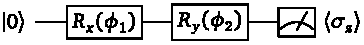
\includegraphics[width=3in]{pics/pennylane}
	\end{center}
	\lstinputlisting[basicstyle=\tiny]{../src/pennylane_example.py}
	\source{arXiv:1811.04968}
\end{frame}
%%%%%%%%%%%%%%%%%%%%%%%%%%%%%%%%%%%%%%%%%%%%%%%%%%%%%%%%%%%%%%%%%%%%%%%%%%%%%%%%
\begin{frame}{Variational quantum algorithm II}
	\begin{figure}
		\centering
		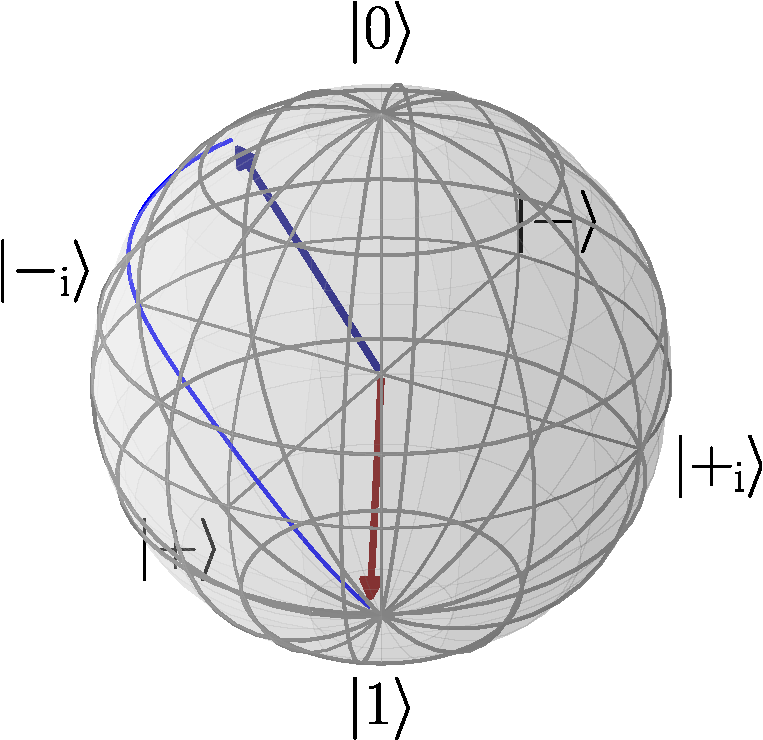
\includegraphics[width=0.3\textwidth]{pics/trajectories/1}
		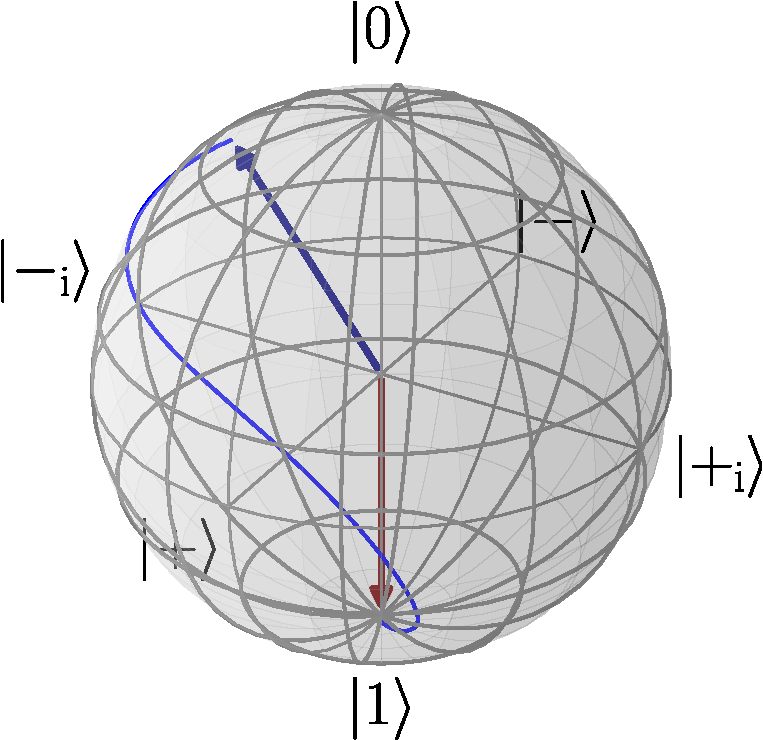
\includegraphics[width=0.3\textwidth]{pics/trajectories/2}
		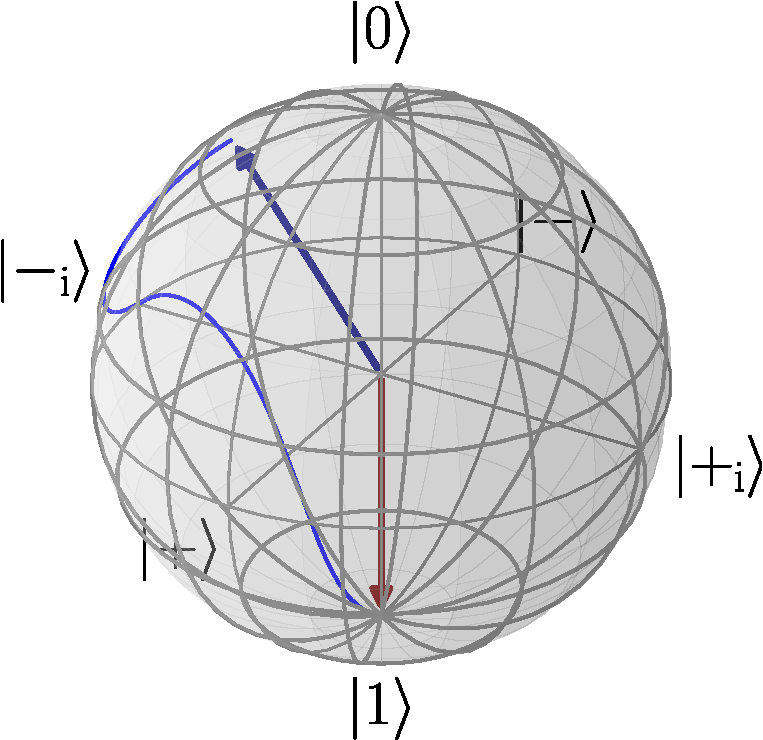
\includegraphics[width=0.3\textwidth]{pics/trajectories/3}
		\caption{Three optimization strategies: gradient descent,
		Nesterov momentum optimizer, Adam optimizer
		($var_\mathrm{init}=(0.5, 0.2)$). }
	\end{figure}
\end{frame}
%%%%%%%%%%%%%%%%%%%%%%%%%%%%%%%%%%%%%%%%%%%%%%%%%%%%%%%%%%%%%%%%%%%%%%%%%%%%%%%%		
\begin{frame}{An example of quantum neural network}
\begin{block}{Dataset}
	We use an artificial dataset (moons) consisting of  two classes.
\end{block}
\begin{block}{Data preprocessing}
	\begin{itemize}
		\item The original feature vectors (single feature for all samples) 
		$X_\mathrm{orig}$ are normalized
		$$X_\mathrm{std} = \frac{X_\mathrm{orig} - \min(X_\mathrm{orig})}
							{\max(X_\mathrm{orig}) - min(X_\mathrm{orig})}$$
		$$X_\mathrm{scaled} = X_\mathrm{std} (\max - \min) + \min,$$
		with $\min = 0$, $\max = \pi$.  
		\item In order to encode as in angle of a qubit rotation.
	\end{itemize}
\end{block}
\end{frame}
%%%%%%%%%%%%%%%%%%%%%%%%%%%%%%%%%%%%%%%%%%%%%%%%%%%%%%%%%%%%%%%%%%%%%%%%%%%%%%%%
\begin{frame}{An example of quantum neural network}
\begin{block}{Data encoding gate}
\begin{itemize}
	\item Encoding gate $U_{\mathrm{e}}(x)$ 
	transforms data sample
	$x=(x_1, x_2, \ldots, x_N)\in \mathbb{R}^N$
	into data state
	$$\ket{x} = U_{\mathrm{e}}(x)\ket{0}^{\otimes N} = 
	R_x(x_1)\otimes R_x(x_2) \otimes \ldots \otimes R_x(x_N) 
	\ket{0}^{\otimes N},
	$$
	\item where 
	$$R_x(\phi) = e^{-i\phi\sigma_x/2} = 
	  \begin{bmatrix}
		\cos(\phi/2) & -i\sin(\phi/2) \\
		-i\sin(\phi/2) & \cos(\phi/2)
	\end{bmatrix}
	$$
	\item and $x_i\in[0,\pi]$.
\end{itemize}
\end{block}
\end{frame}
%%%%%%%%%%%%%%%%%%%%%%%%%%%%%%%%%%%%%%%%%%%%%%%%%%%%%%%%%%%%%%%%%%%%%%%%%%%%%%%%}

%%%%%%%%%%%%%%%%%%%%%%%%%%%%%%%%%%%%%%%%%%%%%%%%%%%%%%%%%%%%%%%%%%%%%%%%%%%%%%%%}
\begingroup
\nologo
\begin{frame}{An example of quantum neural network}
\begin{block}{Variational gate}
\begin{itemize}
	\item Variational gate $U_{\mathrm{v}}(w)$ entangles the information 
	and is parametrized. 
	Angles $w \in \mathbb{R}^{N \times 3 \times L}$ 
	are the parameters we want to learn from the data 
	and $L$ denotes the number of quantum layers.
\end{itemize}
\end{block}
\begin{figure}
	\centering
	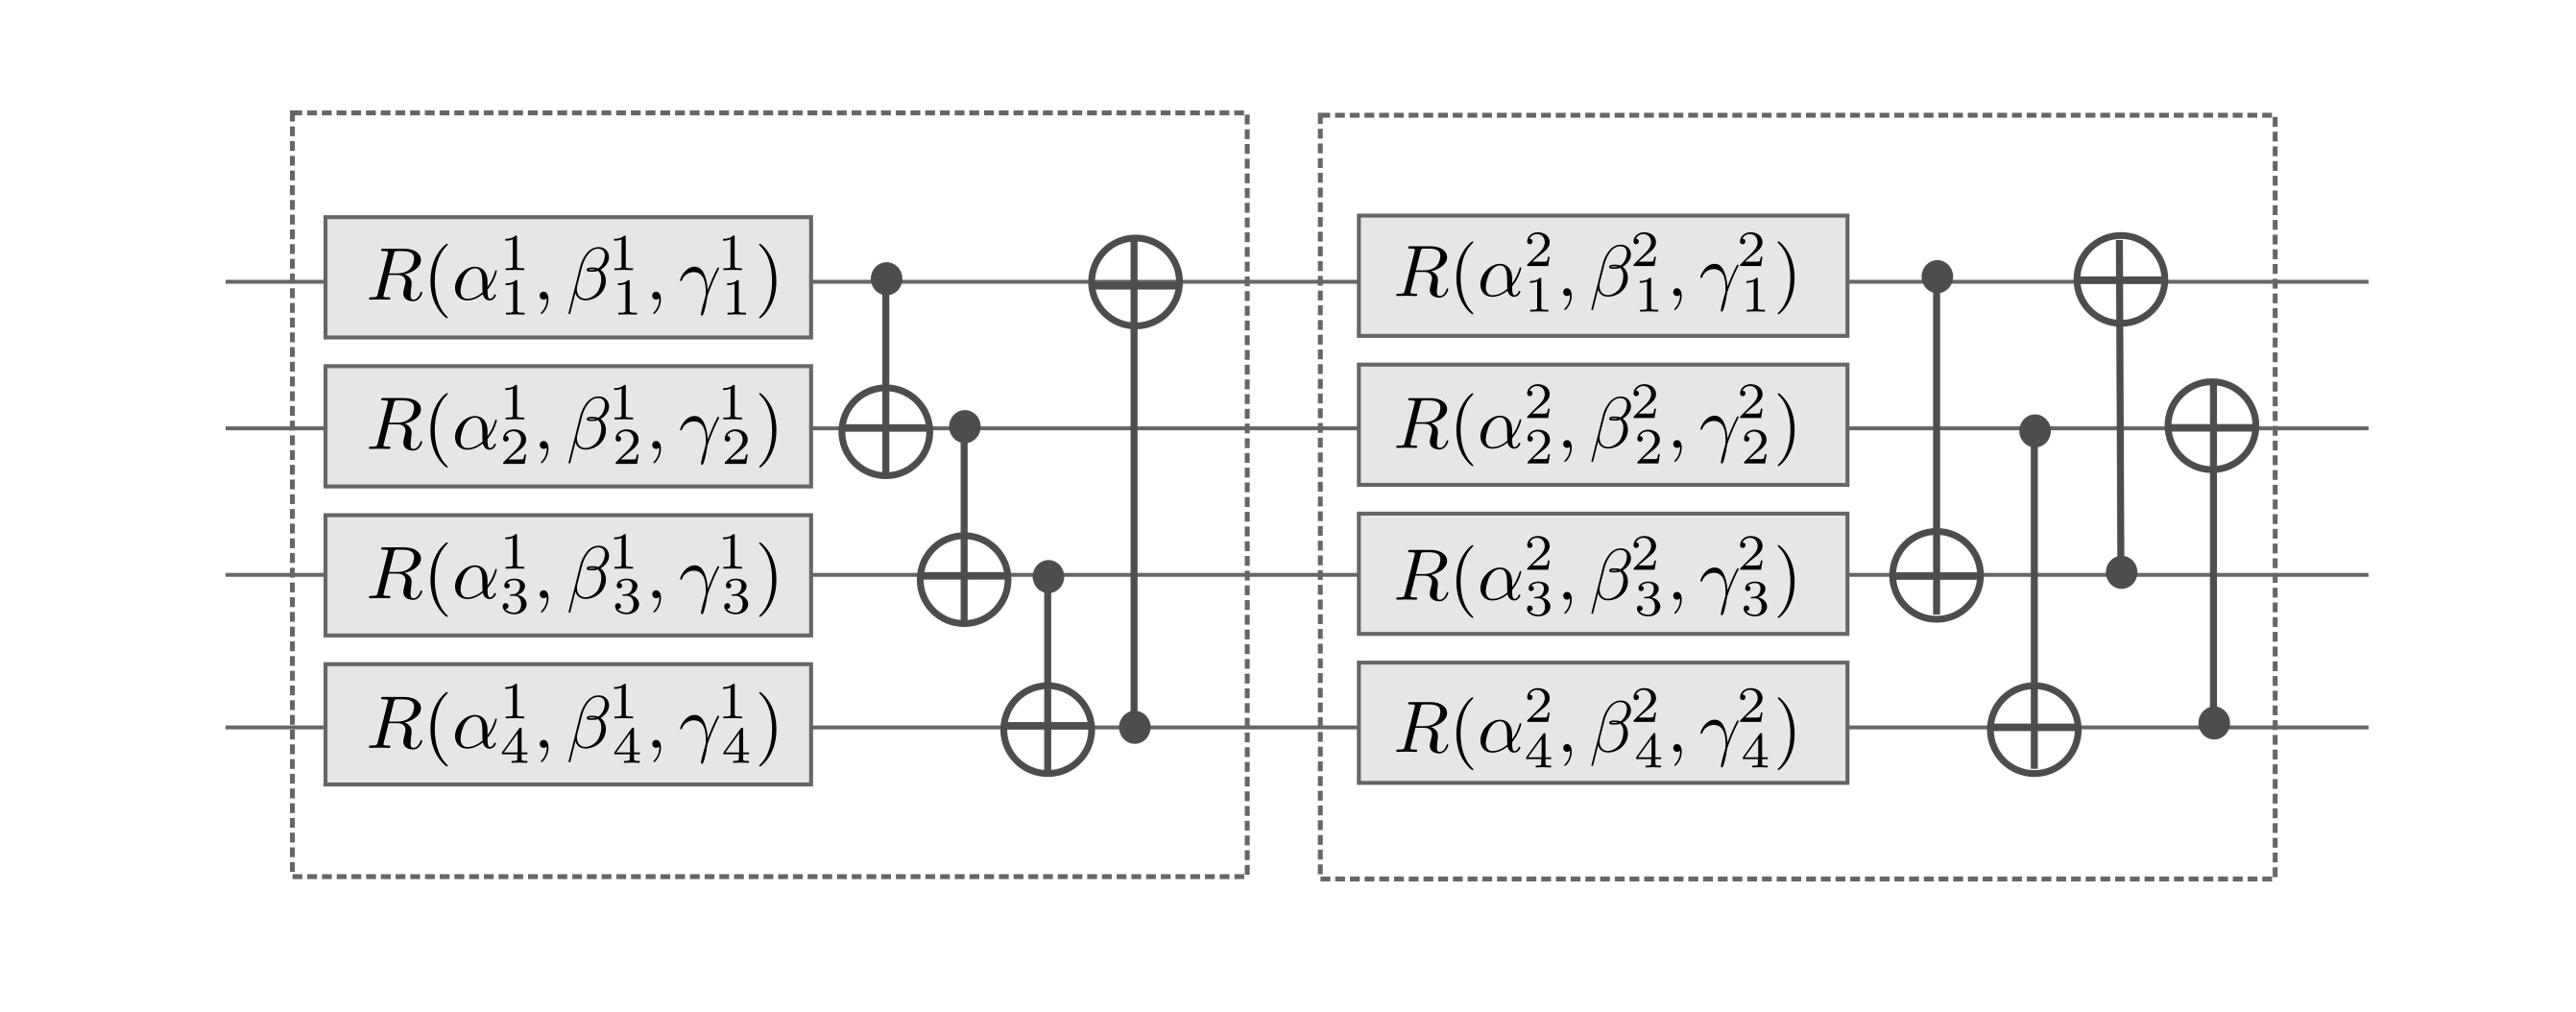
\includegraphics[width=0.8\textwidth]{pics/layer_sec.png}
\end{figure}
\source{https://github.com/XanaduAI/pennylane/ (Distributed under Apache Licence 2.0)}
\end{frame}
\endgroup
%%%%%%%%%%%%%%%%%%%%%%%%%%%%%%%%%%%%%%%%%%%%%%%%%%%%%%%%%%%%%%%%%%%%%%%%%%%%%%%%
\begin{frame}{An example of quantum neural network}
\begin{block}{Decision function}
\begin{itemize}
	\item The decision function $f: \mathbb{R}^N \to \mathbb{R}$.
	\item $f(x; \theta) = 
	\expval{O}_{U_{\mathrm{v}}(\theta) U_{\mathrm{e}}(x)\ket{0}},$
	with
	$$\expval{O}_{U_{\mathrm{v}}(\theta) U_{\mathrm{e}}(x)\ket{0}}=
	\bra{0}U_{\mathrm{e}}(x)^\dagger U_{\mathrm{v}}(\theta)^\dagger  
	O U_{\mathrm{v}}(w) U_{\mathrm{e}}(x)\ket{0},$$
	\item Observable $O= \sigma_z \otimes \mathbb{1}^{\otimes (N-1)} $.
	\item The classification function\\ $\mathrm{cls}: \mathbb{R}^N\to \{-1,1\}$:
	 $\mathrm{cls}(x; \theta) = \mathrm{sgn}(f(x; \theta))$.
\end{itemize}	
\end{block}
\end{frame}
%%%%%%%%%%%%%%%%%%%%%%%%%%%%%%%%%%%%%%%%%%%%%%%%%%%%%%%%%%%%%%%%%%%%%%%%%%%%%%%%
\begin{frame}{An example of quantum neural network}
\begin{block}{Training}
\begin{itemize}
	\item The available data are divided into: train and test.
	\item Initial $\theta$-s: $w\sim\mathcal{U}(0,2\pi)$.
	\item Cost function $$\mathrm{cost}\left(
		(y_i^{\mathrm{train}})_{i\in \xi_t}, 
		(f(X_{i,:}^{\mathrm{train}}; \theta))_{i\in \xi_t}
		\right)
		= \sum_{i\in \xi_t} (y_i^{\mathrm{train}} - f(X_{i,:}^{\mathrm{train}}; \theta))^2/|\xi_t|
		.$$
	\item Batches $\xi_t$.
	% \item In each step use $\theta^{(t)}$ to calculate  
	% $$\mathrm{accuracy}
	% 	\left((y_i^{\mathrm{validation}})_{i}, 
	% 	(\mathrm{cls}(X_{i,:}^{\mathrm{validation}}; \theta^{(t)}))_{i}
	% 	\right).
	% $$
	% \item To avoid over-fitting choose $\theta^{(t)}$ that maximizes accuracy for validation set.
\end{itemize}
\end{block}
\end{frame}
%%%%%%%%%%%%%%%%%%%%%%%%%%%%%%%%%%%%%%%%%%%%%%%%%%%%%%%%%%%%%%%%%%%%%%%%%%%%%%%%
\section{Example in python}
\def\mycode{}
\def\mycolor\color{black}
\def\mylisting<#1>#2#3{\only<#1>{%
	\lstinputlisting[basicstyle=\tiny, language=Python, keywordstyle=\color{teal}\bfseries, firstline=#2, lastline=#3, firstnumber=#2]%
	{\mycode}}}
%%%%%%%%%%%%%%%%%%%%%%%%%%%%%%%%%%%%%%%%%%%%%%%%%%%%%%%%%%%%%%%%%%%%%%%%%%%%%%%%
\subsection{Source code}
%%%%%%%%%%%%%%%%%%%%%%%%%%%%%%%%%%%%%%%%%%%%%%%%%%%%%%%%%%%%%%%%%%%%%%%%%%%%%%%%
\begin{frame}{Binary classification in pennylane}
	\renewcommand{\mycode}{../src/tutorial.py}
	\renewcommand{\mycolor}{\color{yellow!30!white}}
	\begin{block}{%
		\only<1>{Imports}
		\only<2>{Data import, preprocessing and splitting}
		\only<3>{Building the quantum classifier}
		\only<4>{Training preparation}
		\only<5>{Training}
		\only<6>{Inference}
		}
	\mylisting<1>{1}{14}
	\mylisting<2>{17}{30}
	\mylisting<3>{32}{54}
	\mylisting<4>{56}{75}
	\mylisting<5>{76}{91}
	\mylisting<6>{93}{98}
	\end{block}
\end{frame}
%%%%%%%%%%%%%%%%%%%%%%%%%%%%%%%%%%%%%%%%%%%%%%%%%%%%%%%%%%%%%%%%%%%%%%%%%%%%%%%%
\subsection{Visualization of learning process}
%%%%%%%%%%%%%%%%%%%%%%%%%%%%%%%%%%%%%%%%%%%%%%%%%%%%%%%%%%%%%%%%%%%%%%%%%%%%%%%%
\begin{frame}{Learning process}
	\foreach \n [count=\ni] in {1,...,10,15,20} {%
		\only<\ni>{%
			\begin{center}
				{\normalsize Learning step $\n$}\\
				\includegraphics[page=\n, height=0.8\textheight]{pics/qnn/moons}
			\end{center}
		}
	}
\end{frame}